\documentclass[aspectratio=169,10pt]{beamer}

\usetheme{default}
\usepackage[utf8]{inputenc}
\usepackage{graphicx}
\usepackage{booktabs}
\usepackage{tikz}
\usepackage{pgfplots}
\usepackage{xcolor}
\usetikzlibrary{arrows.meta, positioning}
\pgfplotsset{compat=1.18}

% -- Colours --
\definecolor{darkblue}{RGB}{10,45,100}
\definecolor{accent}{RGB}{210,70,20}
\definecolor{lightbg}{RGB}{244,247,255}
\definecolor{greendone}{RGB}{30,130,60}

% -- Beamer --
\setbeamercolor{frametitle}{bg=darkblue, fg=white}
\setbeamercolor{itemize item}{fg=accent}
\setbeamercolor{block title}{bg=darkblue, fg=white}
\setbeamercolor{block body}{bg=lightbg, fg=darkblue}
\setbeamertemplate{itemize item}{$\blacktriangleright$}
\setbeamertemplate{navigation symbols}{}
\setbeamertemplate{footline}{%
  \hfill\tiny\color{darkblue!50}\insertframenumber\hspace{6pt}\vspace{3pt}}
\setbeamerfont{frametitle}{series=\bfseries, size=\normalsize}
\setbeamerfont{block title}{series=\bfseries, size=\small}
\setbeamerfont{block body}{size=\footnotesize}
\setbeamersize{text margin left=7mm, text margin right=7mm}

% -- Simple TikZ box style --
\tikzstyle{pbox}=[rectangle, rounded corners=3pt, draw=darkblue,
  fill=lightbg, font=\tiny\bfseries, text centered, align=center,
  minimum width=1.8cm, minimum height=0.6cm, text=darkblue]
\tikzstyle{garr}=[-{Stealth[length=4pt]}, thick, color=accent]

% ==========================================================
\begin{document}

% ----------------------------------------------------------
% TITLE
% ----------------------------------------------------------
{
\setbeamercolor{background canvas}{bg=darkblue}
\begin{frame}[plain]
  \centering
  \vspace{0.8cm}
  {\tiny\color{white!55}INDIAN INSTITUTE OF INFORMATION TECHNOLOGY, LUCKNOW}\\[0.35cm]
  \rule{0.45\linewidth}{0.3pt}\\[0.4cm]
  {\large\bfseries\color{white}
    A Data-Driven Framework for Wind Energy\\[0.2em]
    Deviation Penalty Optimization}\\[0.5cm]
  \rule{0.45\linewidth}{0.3pt}\\[0.4cm]
  {\small\color{white!85}\textbf{Tapas Barman} \quad MSD24021}\\[0.1cm]
  {\footnotesize\color{white!70}MSc.\ Data Science $\cdot$ Dept.\ of Mathematics}\\[0.25cm]
  {\footnotesize\color{white!65}
    Supervisor: \textbf{Dr.\ Sirsendu Sekhar Barman} \quad March 2026}
\end{frame}
}

% ----------------------------------------------------------
% SLIDE 1 — INTRODUCTION
% ----------------------------------------------------------
\begin{frame}{1. \; Introduction}
  \begin{columns}[T]
    \column{0.55\textwidth}
      \textbf{\color{darkblue}\small India's Renewable Energy Context}\\[5pt]
      \begin{itemize}\setlength\itemsep{5pt}\small
        \item India targets \textbf{500 GW} of clean energy by 2030
        \item Wind power is critical but \textbf{unpredictable} --- depends on weather
        \item Poor forecast $\rightarrow$ wrong schedule $\rightarrow$ \textbf{financial penalties}
      \end{itemize}
      \vspace{8pt}
      \textbf{\color{darkblue}\small The Grid Scheduling Requirement}\\[5pt]
      \begin{itemize}\setlength\itemsep{5pt}\small
        \item All farms must declare output in \textbf{96 slots of 15 min each} daily
        \item Schedule submitted \textbf{1.5--2 hours} before each slot
        \item Deviation from the schedule triggers \textbf{CERC DSM charges}
      \end{itemize}

    \column{0.40\textwidth}
      \centering\vspace{0.5cm}
      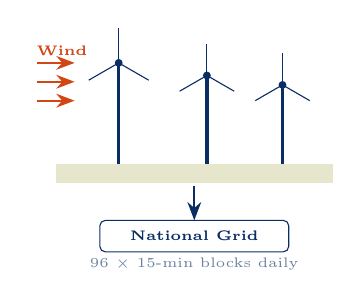
\begin{tikzpicture}[scale=0.80]
        % Turbine 1
        \draw[darkblue, line width=1.2pt] (0.8,0.3) -- (0.8,1.9);
        \draw[darkblue] (0.8,1.9) -- ++(90:0.55);
        \draw[darkblue] (0.8,1.9) -- ++(210:0.55);
        \draw[darkblue] (0.8,1.9) -- ++(330:0.55);
        \filldraw[darkblue] (0.8,1.9) circle (1.5pt);
        % Turbine 2
        \draw[darkblue, line width=1.2pt] (2.2,0.3) -- (2.2,1.7);
        \draw[darkblue] (2.2,1.7) -- ++(90:0.5);
        \draw[darkblue] (2.2,1.7) -- ++(210:0.5);
        \draw[darkblue] (2.2,1.7) -- ++(330:0.5);
        \filldraw[darkblue] (2.2,1.7) circle (1.5pt);
        % Turbine 3
        \draw[darkblue, line width=1.2pt] (3.4,0.3) -- (3.4,1.55);
        \draw[darkblue] (3.4,1.55) -- ++(90:0.5);
        \draw[darkblue] (3.4,1.55) -- ++(210:0.5);
        \draw[darkblue] (3.4,1.55) -- ++(330:0.5);
        \filldraw[darkblue] (3.4,1.55) circle (1.5pt);
        % Ground
        \fill[green!20!brown!25] (-0.2,0.0) rectangle (4.2,0.3);
        % Wind arrows
        \draw[-{Stealth}, accent, thick] (-0.5,1.3) -- (0.1,1.3);
        \draw[-{Stealth}, accent, thick] (-0.5,1.6) -- (0.1,1.6);
        \draw[-{Stealth}, accent, thick] (-0.5,1.9) -- (0.1,1.9);
        \node[font=\tiny, accent] at (-0.1,2.1) {\textbf{Wind}};
        % Arrow to grid
        \draw[-{Stealth}, darkblue, thick] (2.0,-0.05) -- (2.0,-0.6);
        % Grid box
        \draw[darkblue, rounded corners=2pt]
          (0.5,-1.1) rectangle (3.5,-0.6);
        \node[font=\tiny\bfseries, darkblue] at (2.0,-0.85) {National Grid};
        % Label
        \node[font=\tiny, darkblue!60] at (2.0,-1.3)
          {96 $\times$ 15-min blocks daily};
      \end{tikzpicture}
  \end{columns}
\end{frame}

% ----------------------------------------------------------
% SLIDE 2 — PROBLEM STATEMENT + DSM
% ----------------------------------------------------------
\begin{frame}{2. \; Problem Statement \& DSM}
  \begin{columns}[T]
    \column{0.50\textwidth}
      \begin{block}{What is DSM?}
        \footnotesize
        The \textbf{Deviation Settlement Mechanism (DSM)} is CERC's penalty framework. If actual wind generation deviates by more than \textbf{10\%} from the declared schedule, escalating charges are applied.
      \end{block}
      \vspace{6pt}
      \textbf{\color{darkblue}\small Why Is This Hard?}\\[4pt]
      \begin{itemize}\setlength\itemsep{4pt}\small
        \item Global weather models are designed for large regions, not single farms
        \item Existing average error = \textbf{5.96 MW} --- near the 10\% limit
        \item Evening errors (6--10 PM) cost \textbf{2.5$\times$ more}
        \item Result: Crores of rupees in avoidable annual penalties
      \end{itemize}

    \column{0.46\textwidth}
      \centering
      {\small\textbf{\color{darkblue}DSM Penalty Bands (CERC 2024)}}\\[6pt]
      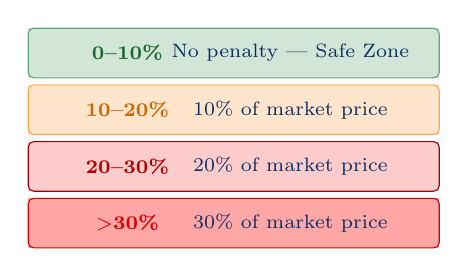
\begin{tikzpicture}[scale=0.90]
        % Band 1 — safe
        \fill[greendone!20] (0,2.4) rectangle (5.8,3.1);
        \draw[greendone!70, rounded corners=2pt] (0,2.4) rectangle (5.8,3.1);
        \node[font=\scriptsize\bfseries, greendone!80!black] at (1.4,2.75) {0--10\%};
        \node[font=\scriptsize, darkblue] at (3.7,2.75) {No penalty — Safe Zone};
        % Band 2
        \fill[orange!20] (0,1.6) rectangle (5.8,2.3);
        \draw[orange!70, rounded corners=2pt] (0,1.6) rectangle (5.8,2.3);
        \node[font=\scriptsize\bfseries, orange!80!black] at (1.4,1.95) {10--20\%};
        \node[font=\scriptsize, darkblue] at (3.7,1.95) {10\% of market price};
        % Band 3
        \fill[red!20] (0,0.8) rectangle (5.8,1.5);
        \draw[red!60!black, rounded corners=2pt] (0,0.8) rectangle (5.8,1.5);
        \node[font=\scriptsize\bfseries, red!70!black] at (1.4,1.15) {20--30\%};
        \node[font=\scriptsize, darkblue] at (3.7,1.15) {20\% of market price};
        % Band 4
        \fill[red!35] (0,0.0) rectangle (5.8,0.7);
        \draw[red!85!black, rounded corners=2pt] (0,0.0) rectangle (5.8,0.7);
        \node[font=\scriptsize\bfseries, red!85!black] at (1.4,0.35) {$>$30\%};
        \node[font=\scriptsize, darkblue] at (3.7,0.35) {30\% of market price};
      \end{tikzpicture}
      \vspace{4pt}
      \footnotesize\color{accent}For 75 MW plant: 10\% = only \textbf{7.5 MW} tolerance
  \end{columns}
\end{frame}

% ----------------------------------------------------------
% SLIDE 3 — CASE STUDY
% ----------------------------------------------------------
\begin{frame}{3. \; Case Study --- RSOPL Koppal, Karnataka}
  \begin{columns}[T]
    \column{0.46\textwidth}
      \textbf{\color{darkblue}\small Site Details}\\[5pt]
      \begin{itemize}\setlength\itemsep{4pt}\small
        \item \textbf{Plant:} RSOPL, Koppal, Karnataka
        \item \textbf{Coordinates:} 15.34°N, 76.15°E
        \item \textbf{Capacity:} 75 MW registered
        \item \textbf{Turbines:} Vestas class, 3 MW, 100 m hub
      \end{itemize}
      \vspace{7pt}
      \textbf{\color{accent}\small 10-Month Financial Audit}\\[5pt]
      \begin{itemize}\setlength\itemsep{4pt}\small
        \item Under-production penalties: \textbf{Rs.\ 41.34 Crores}
        \item Over-production credits: Rs.\ 31.30 Crores
        \item Avg.\ schedule error: \textbf{5.96 MW (7.95\%)}
        \item PI-PML targets cutting this penalty significantly
      \end{itemize}

    \column{0.50\textwidth}
      \centering
      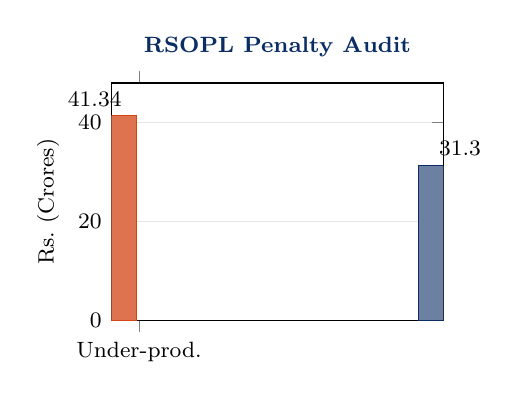
\begin{tikzpicture}
        \begin{axis}[
          ybar, bar width=30pt,
          ylabel={\footnotesize Rs.\ (Crores)},
          symbolic x coords={Under-prod., Over-prod.},
          xtick=data,
          ymin=0, ymax=48,
          nodes near coords,
          nodes near coords style={font=\footnotesize\bfseries},
          width=5.8cm, height=4.6cm,
          tick label style={font=\footnotesize},
          ylabel style={font=\footnotesize},
          ymajorgrids=true, grid style={gray!20},
          title={\footnotesize\bfseries RSOPL Penalty Audit},
          title style={color=darkblue},
        ]
          \addplot[fill=accent!75, draw=accent]
            coordinates {(Under-prod.,41.34)};
          \addplot[fill=darkblue!60, draw=darkblue]
            coordinates {(Over-prod.,31.30)};
        \end{axis}
      \end{tikzpicture}\\[4pt]
      {\footnotesize\color{greendone}\textbf{Rs.\ 41 Crores is our savings target}}
  \end{columns}
\end{frame}

% ----------------------------------------------------------
% SLIDE 4 — MY SOLUTION (Overview)
% ----------------------------------------------------------
\begin{frame}{4. \; My Solution --- PI-PML Framework}
  \centering
  {\small\textbf{\color{darkblue}Physics-Informed Predictive Machine Learning (PI-PML)}}\\[10pt]

  
\begin{tikzpicture}
    \node[pbox, minimum width=2.6cm, minimum height=1.0cm, fill=blue!10]
      (phy) at (0,0) {Physics Engine\\Weather to MW};
    \node[pbox, minimum width=2.6cm, minimum height=1.0cm,
      fill=green!10, draw=green!60!black]
      (ml) at (4.2,0) {XGBoost Model\\Corrects Error};
    \node[pbox, minimum width=2.6cm, minimum height=1.0cm,
      fill=accent!15, draw=accent, text=accent]
      (out) at (8.4,0) {96-Block Schedule\\Sent to CERC};
    \draw[garr, very thick] (phy)--(ml);
    \draw[garr, very thick] (ml)--(out);
    \node[font=\tiny, darkblue] at (0,-0.75) {Step 1: Physics Baseline};
    \node[font=\tiny, darkblue] at (4.2,-0.75) {Step 2: ML Correction};
    \node[font=\tiny, accent] at (8.4,-0.75) {Output: Final Schedule};
  \end{tikzpicture}

  \vspace{0.55cm}
  \begin{columns}
    \column{0.32\textwidth}\centering
      \fcolorbox{darkblue!30}{blue!8}{\parbox{0.88\linewidth}{%
        \centering\footnotesize\color{darkblue}
        \textbf{Input}\\[3pt]
        NOAA GFS weather\\(Wind, Temp, Pressure)}}
    \column{0.32\textwidth}\centering
      \fcolorbox{green!40}{green!8}{\parbox{0.88\linewidth}{%
        \centering\footnotesize\color{darkblue}
        \textbf{Trained on}\\[3pt]
        10 months real SRPC\\generation records}}
    \column{0.32\textwidth}\centering
      \fcolorbox{accent!40}{accent!8}{\parbox{0.88\linewidth}{%
        \centering\footnotesize\color{accent}
        \textbf{Goal}\\[3pt]
        Reduce DSM penalties\\save Crores annually}}
  \end{columns}
\end{frame}

% ----------------------------------------------------------
% SLIDE 5 — SOLUTION DEFINITION
% ----------------------------------------------------------
\begin{frame}{5. \; Solution Definition}
  \begin{columns}[T]
    \column{0.48\textwidth}
      \begin{block}{Physics Engine}
        \begin{itemize}\setlength\itemsep{3pt}
          \item \textbf{Tetens equation} --- humid monsoon air is lighter, less power output
          \item \textbf{Hellman law} --- wind at 100 m is 32\% faster than at 10 m ground level
          \item \textbf{Betz limit} --- turbine extracts at most 59.3\% of wind energy
          \item Rule-based, no training data needed
        \end{itemize}
      \end{block}
    \column{0.48\textwidth}
      \begin{block}{XGBoost Residual Corrector}
        \begin{itemize}\setlength\itemsep{3pt}
          \item Physics still misses: turbine wear, curtailment, local turbulence
          \item \textbf{Residual} = Actual generation $-$ Physics estimate
          \item XGBoost is trained to predict this gap
          \item \textbf{Final:} Physics $+$ XGBoost = corrected schedule
          \item Output clipped to range [0, 75 MW]
        \end{itemize}
      \end{block}
  \end{columns}

  \vspace{0.5cm}
  \centering
  {\small\textbf{\color{darkblue}Forecast Pipeline}}\\[6pt]
  
\begin{tikzpicture}
    \node[pbox, fill=blue!10] (w) at (0,0) {Weather\\Forecast};
    \node[pbox, fill=purple!10, draw=purple!50] (p) at (2.8,0) {Physics\\Baseline};
    \node[pbox, fill=green!10, draw=green!60!black] (e) at (5.6,0) {XGBoost\\Correction};
    \node[pbox, fill=accent!15, draw=accent, text=accent] (f) at (8.4,0) {Final\\Schedule};
    \draw[garr] (w)--(p);
    \draw[garr] (p)--(e);
    \draw[garr] (e)--(f);
  \end{tikzpicture}
\end{frame}

% ----------------------------------------------------------
% SLIDE 6 — DATASET & ARCHITECTURE
% ----------------------------------------------------------
\begin{frame}{6. \; Dataset \& Architecture}
  \begin{columns}[T]
    \column{0.44\textwidth}
      \textbf{\color{darkblue}\small Training Data --- SRPC}\\[5pt]
      \begin{itemize}\setlength\itemsep{4pt}\small
        \item 45 weekly ZIP files from SRPC government portal
        \item Python script auto-extracts all files
        \item \textbf{29,568 blocks}, Apr 2025 -- Feb 2026
        \item Columns: scheduled MW, actual MW, datetime
      \end{itemize}
      \vspace{7pt}
      \textbf{\color{darkblue}\small Live Weather --- NOAA GFS}\\[5pt]
      \begin{itemize}\setlength\itemsep{4pt}\small
        \item Free API, updated \textbf{4 times per day}
        \item Wind at native \textbf{100 m height} (matches turbine hub)
        \item Fetched automatically every morning
      \end{itemize}

    \column{0.53\textwidth}
      \centering
      {\small\textbf{\color{darkblue}System Architecture}}\\[8pt]
      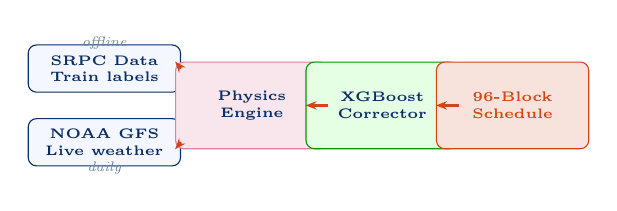
\begin{tikzpicture}[scale=0.72]
        \node[pbox, text width=1.7cm] (srpc) at (0,1.0)
          {SRPC Data\\Train labels};
        \node[pbox, text width=1.7cm] (gfs) at (0,-0.3)
          {NOAA GFS\\Live weather};
        \node[pbox, text width=1.7cm, minimum height=1.1cm,
          fill=purple!10, draw=purple!50]
          (phy) at (2.6,0.35) {Physics\\Engine};
        \node[pbox, text width=1.7cm, minimum height=1.1cm,
          fill=green!10, draw=green!60!black]
          (xgb) at (4.9,0.35) {XGBoost\\Corrector};
        \node[pbox, text width=1.7cm, minimum height=1.1cm,
          fill=accent!15, draw=accent, text=accent]
          (out) at (7.2,0.35) {96-Block\\Schedule};
        \draw[garr] (srpc.east) -- (phy.north west);
        \draw[garr] (gfs.east) -- (phy.south west);
        \draw[garr] (phy)--(xgb);
        \draw[garr] (xgb)--(out);
        \node[font=\tiny\itshape, darkblue!60] at (0.0, 1.45) {offline};
        \node[font=\tiny\itshape, darkblue!60] at (0.0,-0.75) {daily};
      \end{tikzpicture}\\[6pt]
      \begin{tabular}{@{}ll@{}}
        \toprule
        \footnotesize\textbf{Metric} & \footnotesize\textbf{Value}\\
        \midrule
        \footnotesize Total blocks    & \footnotesize 29,568 \\
        \footnotesize Error (before)  & \footnotesize 5.96 MW \\
        \footnotesize Error (after)   & \footnotesize\textbf{1.71 MW} \\
        \footnotesize Improvement     & \footnotesize\textbf{71.2\%} \\
        \bottomrule
      \end{tabular}
  \end{columns}
\end{frame}

% ----------------------------------------------------------
% SLIDE 7 — WORKING
% ----------------------------------------------------------
\begin{frame}{7. \; How It Works}
  \begin{columns}[T]
    \column{0.47\textwidth}
      \textbf{\small\color{darkblue}Phase A --- Training (Done Once)}\\[6pt]
      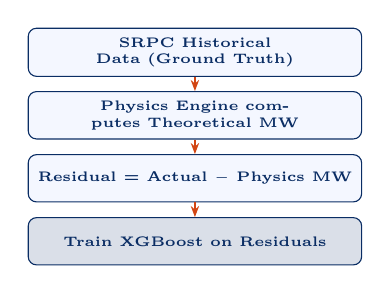
\begin{tikzpicture}
        \node[pbox, text width=4.0cm] (a1) at (0,0)
          {SRPC Historical Data (Ground Truth)};
        \node[pbox, text width=4.0cm] (a2) at (0,-0.80)
          {Physics Engine computes Theoretical MW};
        \node[pbox, text width=4.0cm] (a3) at (0,-1.60)
          {Residual = Actual $-$ Physics MW};
        \node[pbox, text width=4.0cm, fill=darkblue!15] (a4) at (0,-2.40)
          {Train XGBoost on Residuals};
        \draw[garr] (a1)--(a2);
        \draw[garr] (a2)--(a3);
        \draw[garr] (a3)--(a4);
      \end{tikzpicture}

    \column{0.50\textwidth}
      \textbf{\small\color{accent}Phase B --- Upcoming: Live Day-Ahead Pipeline}\\[6pt]
      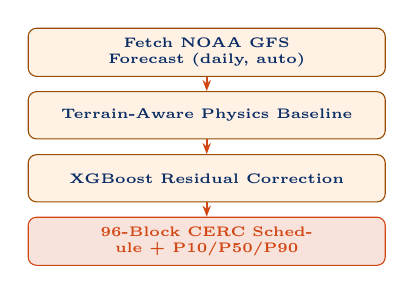
\begin{tikzpicture}
        \node[pbox, text width=4.3cm, fill=orange!10, draw=orange!60!black]
          (b1) at (0,0) {Fetch NOAA GFS Forecast (daily, auto)};
        \node[pbox, text width=4.3cm, fill=orange!10, draw=orange!60!black]
          (b2) at (0,-0.80) {Terrain-Aware Physics Baseline};
        \node[pbox, text width=4.3cm, fill=orange!10, draw=orange!60!black]
          (b3) at (0,-1.60) {XGBoost Residual Correction};
        \node[pbox, text width=4.3cm, fill=accent!15, draw=accent, text=accent]
          (b4) at (0,-2.40) {96-Block CERC Schedule + P10/P50/P90};
        \draw[garr] (b1)--(b2);
        \draw[garr] (b2)--(b3);
        \draw[garr] (b3)--(b4);
      \end{tikzpicture}
  \end{columns}
  \vspace{5pt}
  \footnotesize\color{accent}$\star$ Phase A (training) is complete. Phase B is the upcoming deliverable.
\end{frame}

% ----------------------------------------------------------
% SLIDE 8 — CONCLUSION & FUTURE WORK
% ----------------------------------------------------------
\begin{frame}{8. \; Conclusion \& Upcoming Deliverables}
  \begin{columns}[T]
    \column{0.46\textwidth}
      \textbf{\small\color{darkblue}Work Completed}\\[4pt]
      \begin{itemize}\setlength\itemsep{3pt}\small
        \item CERC DSM 2024 regulatory audit done
        \item \textbf{Dataset 1:} SRPC --- 29,568 blocks collected
        \item \textbf{Dataset 2:} NOAA GFS identified \& tested
        \item Physics Engine built (Tetens, Hellman, Betz)
        \item XGBoost residual model trained \& validated
        \item[\color{greendone}$\star$]
          \textbf{\color{greendone}71.2\% error reduction}
        \item[\color{greendone}$\star$]
          \textbf{\color{greendone}Rs.\ 23.5 Lakhs saved (2-month test)}
      \end{itemize}
      \vspace{5pt}
      \centering
      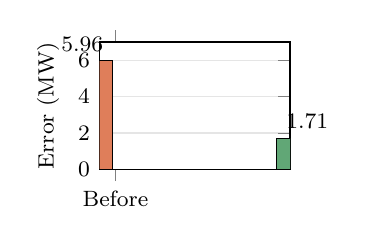
\begin{tikzpicture}
        \begin{axis}[
          ybar, bar width=22pt,
          ylabel={\footnotesize Error (MW)},
          symbolic x coords={Before,After},
          xtick=data, ymin=0, ymax=7,
          nodes near coords,
          nodes near coords style={font=\footnotesize\bfseries},
          width=4.0cm, height=3.2cm,
          tick label style={font=\footnotesize},
          ymajorgrids, grid style={gray!20},
        ]
          \addplot[fill=accent!70] coordinates {(Before,5.96)};
          \addplot[fill=greendone!70] coordinates {(After,1.71)};
        \end{axis}
      \end{tikzpicture}

    \column{0.50\textwidth}
      \textbf{\small\color{darkblue}Upcoming Deliverables}\\[4pt]
      \begin{itemize}\setlength\itemsep{4pt}\small
        \item \textbf{Automated Weather Ingestion:}
          {\footnotesize\ Daily NOAA GFS fetch for Koppal coordinates}
        \item \textbf{Terrain-Aware Wind Correction:}
          {\footnotesize\ Roughness factor for Deccan Plateau hill terrain}
        \item \textbf{Full 96-Block Live Pipeline:}
          {\footnotesize\ Physics $\rightarrow$ XGBoost $\rightarrow$ CERC schedule, automated daily}
        \item \textbf{Probabilistic Output (P10/P50/P90):}
          {\footnotesize\ Risk-adjusted schedule confidence bands}
        \item \textbf{CERC-Formatted Submission:}
          {\footnotesize\ DSM-compliant 96-block day-ahead output}
        \item \textbf{Financial Validation Report:}
          {\footnotesize\ Month-by-month penalty savings vs.= original schedule}
      \end{itemize}
  \end{columns}
\end{frame}

% ----------------------------------------------------------
% THANK YOU
% ----------------------------------------------------------
{
\setbeamercolor{background canvas}{bg=darkblue}
\begin{frame}[plain]
  \centering
  \vspace{1.0cm}
  {\huge\bfseries\color{white}Thank You}\\[0.7cm]
  \rule{0.4\linewidth}{0.4pt}\\[0.5cm]
  {\small\color{white!80}
    A Data-Driven Framework for\\
    Wind Energy Deviation Penalty Optimization}\\[0.5cm]
  {\footnotesize\color{white!65}
    \textbf{Tapas Barman} $\cdot$ MSD24021 $\cdot$ MSc.\ Data Science\\[0.15cm]
    Supervisor: \textbf{Dr.\ Sirsendu Sekhar Barman}\\[0.15cm]
    Department of Mathematics, IIIT Lucknow \quad March 2026}
\end{frame}
}

\end{document}
